The system counts the people entering and leaving a room, presents a classification of the severity of potential queues to enter the room, and sends this information to a web server over a REST api. To be able to do this, a Microsoft Kinect is placed over each entrance to the room, and is connected to the computation device that runs the system software for that room. A debug/configuration GUI can be used to calibrate and configure the software. This produces configuration files that are used by the system. Further tuning and configuration can be done by editing the configuration files. 

\begin{figure}[htb]
	\centering
	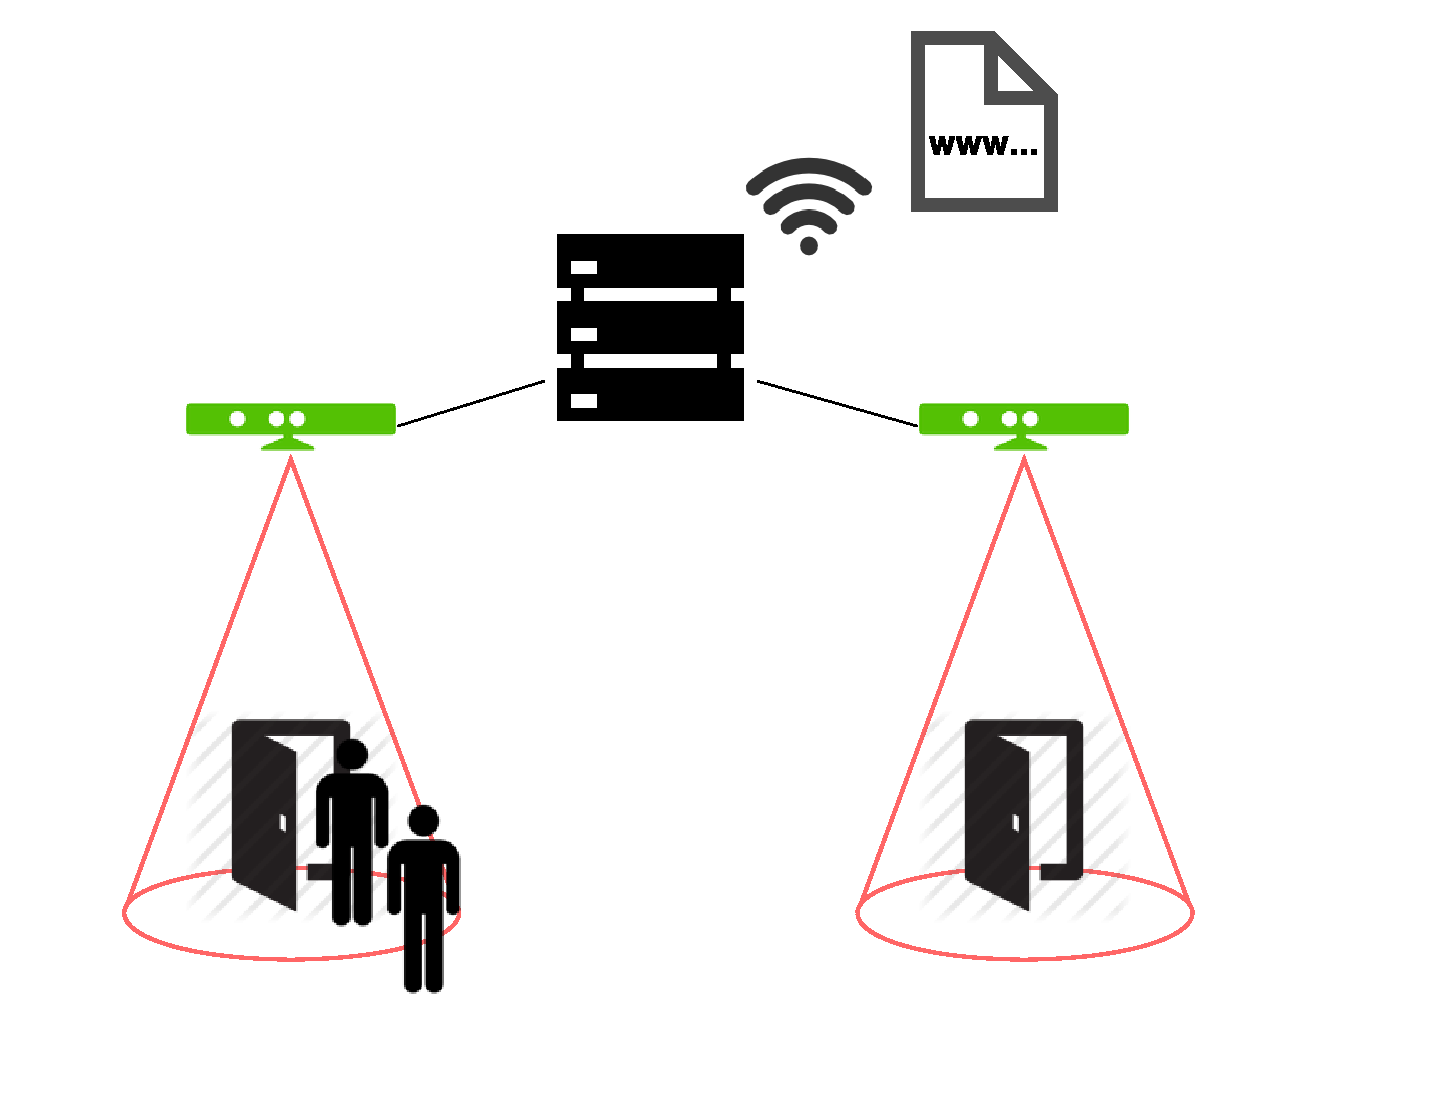
\includegraphics[width=\linewidth]{images/system_overview.pdf}
	\caption[Overview of the entire system]{\textit{System overview.}}
	\label{fig:system_overview}  %Skapar referens till figuren
\end{figure}

\subsection{Platform and hardware requirements}
The system runs and has been tested on Windows, Mac OS X, and Linux. It has  run at real time frame rates on a Linux virtual machine with 512 MB RAM but has not been tested on any embedded devices. It however should work given that the device has sufficient processing power. Care must be taken when considering embedded devices so that the USB module can handle the data volumes needed to stream depth images from the Kinect device at 30 fps. 

\subsection{Configuration}
The whole system can be configured by editing the plain text YAML configuration files. Among other things, it is possible to set what image processing algorithms should be run, in what order to run them and the value of most parameters. Many components in the Debug GUI, camera settings and important file paths are also set in the configuration files. 

\subsection{Modular software architecture}
The software has a modular and easily extendable design, where each module is responsible for a specific domain of the system. The architecture of the system is that of a pipeline of algorithms, where data pertaining to the latest few frames is piped through each pipeline step by the main program. The order is specified in a configuration file and set in place during program initialization. The frame data consists of both raw sensor data and computed data from the different pipeline steps. 

\subsubsection{Network module}
The network module manages all system input/output, i.e. sampling the sensors and posting output data on the web server specified by the configuration file. Currently, support exists for all OpenCV-compatible cameras as well as the Microsoft Kinect depth sensor. The module is designed to be as modular as possible, allowing for a relatively easy integration of new sensor types into the system. The network module also supports running several sensors in parallel. 

\subsubsection{Image processing module}
The image processing module handles all processing that is done directly on any RGB or depth data. This includes detection of objects and object attributes as well as object tracking.

\subsubsection{Statistics module}
The statistics module handles computation and processing that is not done directly on RGB or depth data. This includes counting the number of entering and exiting objects, using object attributes to infer the presence of queues and all data aggregation. 

\subsubsection{Evaluation module}
The evaluation module handles the evaluation of the algorithm pipeline by comparison between its results and the ground truth on labeled data sets.  

\subsection{Debugging and configuration GUI}
The system includes a debugging and configuration GUI where the results from each of the process steps can be viewed in real time, and one step at a time. It can also be used to assist in tuning and calibrating the system, and is necessary for proper set up of a new sensor/room. 
